\documentclass[12pt,dvipdfmx]{book}
\usepackage[margin=1in]{geometry}
\usepackage{amsmath,amssymb,amsfonts,mathtools,amsthm}
\usepackage[dvipdfmx]{graphicx}
\usepackage{tcolorbox,todonotes}
%\usepackage{slashbox}
%\usepackage{wrapfig}
%\usepackage{url,xspace,ascmac}
%\usepackage[]{xcolor}
%\usepackage{tcolorbox,todonotes}
\tcbuselibrary{breakable, skins, theorems}
%\usepackage{svg}
%\usepackage{etoolbox}
%\usepackage[subrefformat=parens]{subcaption}
%\usepackage{algorithm}
%\usepackage{algorithmic}
\usepackage[normalem]{ulem}
\usepackage{comment,tikz}
%\usepackage{todonotes}
%\usepackage{thmtools,thm-restate}
%\usepackage{enumitem}
%\usepackage{ifthen}
%\usepackage{float}

\usetikzlibrary{positioning,calc}

\tikzset{every picture/.style={font issue=\footnotesize},
            font issue/.style={execute at begin picture={#1\selectfont}}
        }

\usepackage[unicode,colorlinks=true,citecolor=blue,linkcolor=blue,pdfusetitle]{hyperref}
\usepackage[style=alphabetic,natbib=true,natbib=true,maxnames=99,maxalphanames=99,isbn=false,url=false,backref=true,backend=biber,giveninits=true]{biblatex}

%\usepackage[style=alphabetic,natbib=true,maxnames=99,maxalphanames=99]{biblatex}
\addbibresource{ref.bib}

\usepackage{cleveref}

\input{theorems.tex}
\newcommand{\defeq}{\mathrel{:=}}
\DeclarePairedDelimiter{\floor}{\lfloor}{\rfloor} % floor function
\DeclarePairedDelimiter{\ceil}{\lceil}{\rceil} % ceil function

\newcommand{\Ver}{\mathrm{Ver}}

\newcommand{\indicator}[1]{\mathbf{1}_{#1}}
\newcommand{\condition}{\;\middle\vert\;}
\newcommand{\tand}{\text{ and }}
\newcommand{\tif}{\text{if }}
\newcommand{\totherwise}{\text{otherwise}}

\newcommand{\e}{\mathrm{e}}
\DeclareMathOperator*{\E}{\mathbb{E}}
\DeclareMathOperator*{\Var}{\mathbf{Var}}
\newcommand{\dtv}{d_{\mathrm{TV}}}
\newcommand{\F}{\mathbb{F}}
\newcommand{\diam}{\mathrm{diam}}
\newcommand{\Fq}{\mathbb{F}_q}
\newcommand{\dist}{\mathrm{dist}}
\newcommand{\Nat}{\mathbb{N}}
\newcommand{\Real}{\mathbb{R}}
\newcommand{\Int}{\mathbb{Z}}
\newcommand{\Comp}{\mathbb{C}}
\newcommand{\binset}{\{0,1\}}
\newcommand{\supp}{\mathsf{supp}\xspace}
\renewcommand{\emph}[1]{\textbf{#1}}
\newcommand{\allone}{\mathbf{1}}
\newcommand{\Cay}{\mathrm{Cay}}

\newcommand{\PRIMES}{\mathrm{PRIMES}}
\newcommand{\ThreeCOL}{\mathrm{3COL}}

\newcommand{\RS}{\mathrm{RS}}
\newcommand{\RM}{\mathrm{RM}}
\newcommand{\Had}{\mathrm{Had}}
\newcommand{\restr}[1]{|_{#1}}

\newcommand{\calA}{\mathcal{A}}
\newcommand{\calB}{\mathcal{B}}
\newcommand{\calC}{\mathcal{C}}
\newcommand{\calD}{\mathcal{D}}
\newcommand{\calE}{\mathcal{E}}
\newcommand{\calF}{\mathcal{F}}
\newcommand{\calG}{\mathcal{G}}
\newcommand{\calH}{\mathcal{H}}
\newcommand{\calI}{\mathcal{I}}
\newcommand{\calJ}{\mathcal{J}}
\newcommand{\calK}{\mathcal{K}}
\newcommand{\calL}{\mathcal{L}}
\newcommand{\calM}{\mathcal{M}}
\newcommand{\calN}{\mathcal{N}}
\newcommand{\calO}{\mathcal{O}}
\newcommand{\calP}{\mathcal{P}}
\newcommand{\calQ}{\mathcal{Q}}
\newcommand{\calR}{\mathcal{R}}
\newcommand{\calS}{\mathcal{S}}
\newcommand{\calT}{\mathcal{T}}
\newcommand{\calU}{\mathcal{U}}
\newcommand{\calV}{\mathcal{V}}
\newcommand{\calW}{\mathcal{W}}
\newcommand{\calX}{\mathcal{X}}
\newcommand{\calY}{\mathcal{Y}}
\newcommand{\calZ}{\mathcal{Z}}

\title{PCP定理とその証明}
\author{清水 伸高 (東京科学大学)}
\date{}
\begin{document}
\maketitle
\tableofcontents
\chapter*{序文}



このノートは, 京都大学大学院理学研究科数学・数理解析専攻数理解析系の数理解析特別講義Ⅰにおける集中講義「PCP定理の証明と応用」の講義ノートである.
計算量(computational complexity)とは, 問題を解くために必要な計算リソースの量(例えば計算時間, 記憶領域のサイズ, 乱択や量子性の有無や量)を意味し, 計算量理論(computational complexity theory)とはそれぞれの問題の計算量を明らかにするための理論である.
PCP定理とは, 判定問題(YesかNoで答える問題)の検証に要する計算量に関する結果であり,
端的に言うと, ある命題が真であると主張する証明が文字列として与えられたとき,
その証明を検証するためには, 通常, 全ての文字を見て確認する必要があるが,
PCP定理によれば, その証明の一部だけを見ることで, その命題が真であるか否かを確率的に検証することができるという驚くべき結果である.
例えば, ある実行列$A$と実ベクトル$b$に対して線形方程式系$Ax=b$は解を持つ, という命題を考えてみよう.
この命題が真であるならば実際に解の一つ$x$を証明として提示することができるが, その証明が正しいかどうかを検証するためには検証者は$Ax$を実際に計算し, その各成分が$b$と一致するかを確認する必要がある.
ところがPCP定理によれば, 巧妙に構成された証明$\pi$を提示することにより, その証明$\pi$全ての文字を見ることなく, 99\%の確率で正しく検証できるのである (ここでは確率的な検証, つまり検証者はランダムネスを用いた検証を行う設定を考える).

このように, 局所的な情報だけを使って全体の構造を推測できるというPCP定理の性質は, 単に理論的に興味深いだけでなく, 誤り訂正符号の構成, 確率論的手法の脱乱択化, 最適化問題の近似率限界の導出など, 理論計算機科学において広大な応用を持ち, 現在でも計算量理論の中心的な研究対象の一つである.
このような重要性を持つにもかかわらず, PCP定理の証明に包括的に日本語でアクセスできる文献は(筆者が知る限り本資料の執筆時点では)存在しない.
本講義ではPCP定理の証明を与えるとともに, その証明に用いられた計算量理論の基本的な概念や技法を解説し,
PCP定理の応用についても触れる.
僭越ながらもこれはPCP定理の証明に日本語でアクセスする(おそらく国内初の)資料であるといえる.
今回のような挑戦的な機会を与えてくださった河村彰星先生に感謝を申し上げる.

\addcontentsline{toc}{chapter}{Preface}
\chapter{導入}

この集中講義ではPCP定理と呼ばれる計算量理論の基本的な結果について解説し, その証明を与える.
PCP定理は1998年に\citet{AroraS98,AroraLMSS98}によって証明された.
この証明は代数的な手法に基づく誤り訂正符号を技巧的に組合せたものであり, 難解なものであったが, その後\citet{Din07}によってより簡潔な証明が与えられた.
この講義では\citet{Din07}による比較的簡単な証明を紹介する.
ちなみにDinurはのちにこの業績によりゲーデル賞を受賞している.

\section{計算量理論の復習}
まずは計算量理論のどの教科書にも載っているような基礎的な用語の定義を与える. これらの用語に明るい読者は\cref{sec:PCP}から読み始めても良い.
なお, このノートではアルゴリズムの定義 (チューリング機械の定義) は省略し, アルゴリズムについて述べる際は具体的な計算の手続きを述べる\footnote{ひとまずPythonやC言語などで実装されたプログラムを考えれば良い. ただし, 計算機内では全ての数値は有限桁の二進数で表記されており, その読み書きや演算には少なくとも桁数に比例した計算時間がかかる. なお, $\sqrt{2}$といった無理数は本来は有限桁で打ち切った近似値を扱うが, そのような小数はこの講義では扱わず, 特に断りのない限りは整数値のみを考える. また, 記憶領域へのアクセスは定数時間で行えると仮定する(チューリング機械であればテープの移動にかかる時間も考慮する).}.

まずは基本的な記号の定義を与える:
\begin{itemize}
\item オーダー記法: 二つの関数$f,g\colon\Nat\to\Nat$に対し, $f(n)=O(g(n))$であるとは, ある定数$c>0$が存在して, 十分大きな全ての$n\in\Nat$に対して$f(n)\le cg(n)$が成り立つことをいう. また, $f(n)=\Omega(g(n)), f(n)=o(g(n)), f(n)=\omega(g(n))$なども同様に($n\to\infty$として)定義する.
\item 自然数$n\in\Nat$に対して$[n]=\qty{1,\dots,n}$とする.
\item 有限集合$S$に対し, $x\sim S$と書いたとき, $x$は$S$から一様ランダムに選ばれた元であることを意味する.
\item 集合$S$上のベクトル$x\in S^n$および$I\subseteq[n]$に対し, $x_I \in S^I$を, $x$の$I$への制限, すなわち, $x_I(i)=x(i)$ ($i\in I$) と定義する.
\item 本資料で登場する全ての有限集合$S=\{s_1,\dots,s_m\}$に対し$s_1<s_2<\dots<s_m$という順序が暗に定まっているとする. 非空な部分集合$T=\qty{t_1,\dots,t_k}\subseteq S$を考える際は常にこの順序に従って$t_1<\dots<t_k$を仮定する. 例えばグラフの頂点集合にも順序が一つ決まっており, 無向辺$e=\{u,v\}$を考える際も\emph{常に}$u<v$を仮定する.
\item $\binset^*=\bigcup_{n\in\Nat}\binset^n$を有限長の二進文字列全体とする.
\item $x\in\binset^*$に対して$\abs{x}$を$x$の文字数とする.
\item アルゴリズム$A$に対し, $A(x)$を入力$x \in \binset^*$に対するアルゴリズム$A$の出力とする. ここで, 単に「アルゴリズム」と言った場合は決定的アルゴリズムを指し, 乱択アルゴリズムについては明示的に言及する.
\item 関数$T(n)\colon\Nat\to\Nat$を考える. 十分大きな全ての$n\in\Nat$と全ての$x\in\binset^n$に対して, $A$が$A(x)$を出力するまでにかかる計算ステップ数の最大値が高々$T(n)$であるとき, アルゴリズム$A$の計算量は$T(n)$であるという. 特に, ある($n$に依らない)定数$c>0$が存在して計算量が$O(n^c)$で抑えられるアルゴリズムを\emph{多項式時間アルゴリズム}という\footnote{計算モデルによって一つ一つの計算ステップの定義は異なるが, 原理的には1bitの演算や記憶領域への読み書きの回数と思えばよい. 多項式時間で動くかどうかの議論であれば, 多くの古典的な計算モデルは等価である.}
\item 計算量理論において慣例的に用いられる記法だが, 関数$f(n)$が$n$に関する多項式である, すなわち$n$に依存しないある定数$c>0$に対して$f(n)=O(n^c)$が成り立つことを$f(n)=n^{O(1)}$または$f(n)=\poly(n)$と表す. 例えば多項式時間アルゴリズムとは, 十分大きな全ての$n\in\Nat$に対して, 長さ$n$の任意の文字列$x\in\binset^n$を受け取ったときの時間計算量が$n^{O(1)}$で抑えられるアルゴリズムである.
\item 二つの文字列$x,y\in\binset^*$を入力として受け取るアルゴリズムは$A(x,y)$と表す. 三つ以上の場合も$A(x,y,z)$などと表す.
\end{itemize}

計算量理論で最も基本的な問題群として判定問題と呼ばれる問題群がある.

\begin{definition}{判定問題}{decision-problem}
  部分集合$L\subseteq\binset^*$を\emph{判定問題(または言語)}といい,
  アルゴリズムに与える$L$の入力を\emph{インスタンス}という.
  また, インスタンス$x\in\binset^*$は$x\in L$であるとき, 判定問題$L$の\emph{Yesインスタンス}といい,
  そうでない場合は\emph{Noインスタンス}という.

  文字列$x\in\binset^*$に対し$L(x)\in\binset$を, $x\in L$かどうかの指示関数, すなわち$x\in L$ならば$L(x)=1$, そうでなければ$L(x)=0$と定義する.

  アルゴリズム$A$は, 任意の$x\in\binset^*$に対して$A(x)=L(x)$が成り立つとき,
  $A$は$L$を解くという.
\end{definition}

\begin{example}{グラフ連結性判定問題}{graph-connectivity-problem}
  グラフ$G=(V,E)$の隣接行列を$A \in \binset^{|V|\times|V|}$とする.
  この行列を長さ$|V|^2$の二進文字列として表現したものを$\mathsf{str}(A)$とする.
  すなわち, $\mathsf{str}(A)$の第$k$ビットは, $i=\ceil{k/|V|}+1, j=k\mod |V|+1$に対して$A(i,j)$の値として与えられる.
  このとき,
  \begin{align*}
    L = \qty{ \mathsf{str}(A)\in\binset^{|V|^2} \colon \text{$A$は連結グラフ$G$の隣接行列} }
  \end{align*}
  は与えられたグラフが連結であるかどうかを判定する判定問題である.
\end{example}

この講義では「効率的に解ける」といった場合, 多項式時間アルゴリズムによって解けることを指す. そのような判定問題の集合をクラスPという.
\begin{definition}{クラスP}{classP}
  判定問題$L$は, それを解く多項式時間アルゴリズムが存在するとき, $\P$に属するといい, $L \in \P$と表す.
\end{definition}

\begin{remark}{入力のフォーマット}{input-format}
  \cref{ex:graph-connectivity-problem}では入力としてグラフの隣接行列を二進文字列として表現したものを考えたが, 一般にグラフの表現方法は他にも隣接リストなどが考えられる.
  しかし, 例えばグラフを隣接行列で表現するか隣接リストで表現するかは, それぞれのフォーマット間の変換が多項式時間で行えるため, \emph{多項式時間で解けるかどうか}という点では等価である.

  そのため, 厳密には問題を定義する際はその入力のフォーマット(グラフを隣接行列で表現するか, 隣接リストで表現するか, など)も指定する必要があるが,
  フォーマット間の変換が自明に多項式時間で行える場合に限ってはこの講義ではそのようなフォーマットの指定を省略し, 例えばグラフ連結性判定問題を「グラフが与えられたときにそれが連結であるかどうかを判定する問題」と表現する.
\end{remark}

次に乱択アルゴリズムについて定義する. 端的に言えばアルゴリズムの内部でコイントスを行うものを乱択アルゴリズムという.
ここでは明示的にランダムシードを受け取るアルゴリズムを乱択アルゴリズムと呼ぶことにする.

\begin{definition}{乱択アルゴリズム}{randomized-algorithm}
  入力$x\in\binset^*$とは別にランダムシード(乱数表)と呼ばれる別の文字列$s\in\binset^*$を受け取るアルゴリズムを\emph{乱択アルゴリズム}といい, ランダムシードであることを強調するために$A(x;s)$などと表す.
  なお, 任意の$x,s\in\binset^*$に対して$A(x;s)$は有限時間で停止するとし, その計算量は$\abs{x}$のみに依存する関数で表せるとする.
  このとき, ランダムシード$s$の長さを常に$A$の計算量で上から抑える.
  すなわち, $A$の計算量が$T(n)$であるとき, 十分大きな全ての$n\in\Nat$と全ての$x\in\binset^n$に対して$A$が読み込む$s$の文字数は高々$T(n)$であるため, $s\in \binset^{T(n)}$であると仮定する.
  しばし, ランダムシード$s$を明記する必要が特にない場合は$A(x)$と表す.

  乱択アルゴリズムのランダムシードに関する確率, 期待値, 分散を議論する際は記号として$\Pr_{A}[\cdot],\E_A[\cdot],\Var_A[\cdot]$を用いる.
  乱択アルゴリズム$A$が判定問題$L$を解くとは,
  \begin{align*}
    \Pr_A[A(x)=L(x)]\geq 2/3
  \end{align*}
  が成り立つことをいう.
\end{definition}

また, 入力とは別に文字列へのオラクルアクセスを受け取るアルゴリズムを考える.
\begin{definition}{オラクルアルゴリズム}{oracle-algorithm}
  文字列$\pi\in\binset^*$に対し, $\pi$への\emph{オラクルアクセス}を持つアルゴリズム$A^\pi(x)$とは, 計算途中で$\pi$の指定された位置の文字を読むことができるアルゴリズムである.
  すなわち, $\pi$の$i$番目の文字を読む操作を$A^\pi(x)$の計算過程中に$O(\log \abs{\pi})$時間で行うことができるアルゴリズムである.\footnote{自然数$i\in[\abs{\pi}]$を指定するために$O(\log \abs{\pi})$ビットを定めなければならないため, $O(\log \abs{\pi})$時間を仮定している.}
  同様に乱択オラクルアルゴリズムについても定義できる.
\end{definition}


\section{検証の計算量}
数学全般における検証とは, ある命題が真であると主張する証明が与えられたとき, その証明が実際に
その命題を正しく証明しているかどうかを確認することを意味する.
論文や記述試験の証明の査読や採点をイメージしてもらうとわかりやすいだろう.
計算量理論では検証やその計算量の議論は重要な研究テーマであり, その検証に要する計算量が議論される.

\subsection{効率的な検証とクラスNP}
判定問題$L$と入力$x\in\binset^*$を与えられたとき, $x\in L$かどうかを審議したい.
ここで$x\in L$を主張する証明が文字列$\pi\in\binset^*$で与えられたとする.
このとき, \emph{検証者}と呼ばれるアルゴリズムは$x$と$\pi$を読み込んで$x\in L$かどうかを判定する.
この判定を多項式時間で行えるとき, その判定問題$L$の集合を$\NP$という.

\begin{definition}{クラスNP}{classNP}
  判定問題$L$は, 以下を満たす多項式時間アルゴリズム$V$と多項式$p\colon\Nat\to\Nat$が存在するとき, $L$は$\NP$に属するという:
  アルゴリズム$V$は入力として$x,\pi\in\binset^*$を受け取り, $0$または$1$を出力する.
  \begin{enumerate}
  \item もし$x\in L$ならば, ある$\pi\in\binset^{p(\abs{x})}$が存在して$V(x,\pi)=1$となる.
  \item もし$x\notin L$ならば, 全ての$\pi\in\binset^{p(\abs{x})}$に対して$V(x,\pi)=0$となる.
  \end{enumerate}
  また, このようなアルゴリズム$V$を\emph{NP検証者}といい, $\pi$を\emph{NP証明}という.
\end{definition}

\begin{remark}{クラスPとNPの関係}{remark.P-NP}
  判定問題$L$が$\P$に属するならば$L\in\NP$である.
  実際, 受け取った$x\in\binset^*$に対して$L(x)$を計算してそれを出力する検証者を考えばよい.
  すなわち$\P\subseteq\NP$である.
  一方, 逆側の包含関係$\NP\subseteq\P$が成り立つかどうかはP vs NP問題と呼ばれる計算量理論における最も重要な未解決問題であり, 多くの研究者は$\NP\subseteq\P$が成り立たないと信じている.
\end{remark}

検証者$V(x,\pi)$が$1$を出力したとき, $V$は証明$\pi$を\emph{受理する}といい,
検証者が$0$を出力したとき, $V$は証明$\pi$を\emph{拒否する}という.

\begin{example}{合成数判定問題}{composite-number-problem}
  判定問題$L=\{x\in\binset^*\colon x\text{は合成数}\}$を考える.
  このとき, 検証者は$x$と$\pi$を読み込んで, $\pi\not\in\{1,x\}$かつ$\pi$が$x$を割り切るかどうかを判定する.
  もしも$x\in L$である場合, 合成数なので非自明な約数を証明$\pi$として与えれば$V(x,\pi)=1$となる.
  そうでない場合, 非自明な約数は存在しないため必ず$V(x,\pi)=0$となる.
  このアルゴリズム$V$は入力長(つまり数値の二進表現したときのビット長)に関する多項式時間で動作するため, $L$はNPに属する.
\end{example}

\begin{example}{グラフ彩色問題}{graph-coloring-problem}
  自然数$k\ge 2$とグラフ$G=(V,E)$に対し, 関数$c\colon V\to[k]$が
  全ての辺$\{u,v\}\in E$に対して$c(u)\neq c(v)$を満たすとき, $c$を$G$の$k$-彩色といい,
  $k$-彩色が存在するようなグラフは$k$-彩色可能であるという.
  任意の$k\ge 2$に対し, 判定問題
  $$L=\{G\in\binset^*\colon G\text{は}k\text{-彩色可能}\}$$
  はNPに属する.
  検証者は$G$と$\pi$を読み込んで, $\pi$が$G$の$k$-彩色であるかどうかを判定する.
  もしも$G\in L$である場合, $G$は$k$-彩色可能であるため, $k$-彩色の証明$\pi$を与えれば$V(G,\pi)=1$となる.
  そうでない場合, $G$は$k$-彩色可能でないため必ず$V(G,\pi)=0$となる.
  このアルゴリズム$V$は多項式時間で動作するため, $L$はNPに属する.
\end{example}

\begin{exercise}{素数判定問題}{exer.prime-problem}
  自然数$n\in\Nat$に対しその二進表記を$(n)_2\in\binset^*$と表す.
  判定問題$\PRIMES=\{(a)_2\in\Nat\colon a\text{は素数}\}$を考える.
  この問題は$\P$に属することが知られている\cite{AKS04}が, その複雑なアルゴリズムを用いずに
  初等的に$\PRIMES\in \NP$を示したい.
  そのために, 以下の事実を用いる:

  任意の自然数 $a\in\Nat$と$\gamma\in\{1,\dots,a-1\}$に対し, $\gamma^0,\gamma^1,\dots \pmod a$は周期的である. さらに, 以下が成り立つ:
  \begin{itemize}
  \item $a$が素数であるならば, ある$\gamma\in\{1,\dots,a-1\}$が存在して$\gamma^0,\gamma^1,\dots \pmod a$の周期が$a-1$である\footnote{このような$\gamma$を原始元という.}.
  \item 一方, $a$が素数でないならば, 全ての$\gamma\in\{1,\dots,a-1\}$に対して$\gamma^0,\gamma^1,\dots \pmod a$の周期は$a-1$未満である. 特に, その周期$L$は$a-1$を割り切る.
  \end{itemize}
  これらの事実を用いて, 以下の小問に答えよ.

  \begin{enumerate}
  \item 次の検証者$V_1$を考える: 入力$a\in\Nat$と証明$\gamma\in\{1,\dots,a-1\}$に対し, $\gamma^0,\gamma^1,\dots,\gamma^{a-2} \pmod a$を全て検証し, これら全て相異なるかどうかを判定する. この検証者$V_1$が多項式時間アルゴリズム\emph{でない}理由を簡潔に説明せよ.
  \item 入力$a\in\Nat$に対し, $a$が素数であることの証明として, 原始元$\gamma\in\{1,\dots,a-1\}$および$a-1$の素因数分解$a-1=p_1^{\alpha_1}\cdots p_k^{\alpha_k}$および各$p_i$が素数であることの証明を再帰的に与える. この証明を用いて, 検証者$V_2$は$a$が素数であるかどうかを多項式時間で判定できることを示せ.
  \end{enumerate}
\end{exercise}

\subsection{局所的な検証とクラスPCP} \label{sec:PCP}

一般に$x\in L$かどうかの検証では, 証明$\pi$の全ての文字を読む必要がある.
しかし, 証明$\pi$のうちの一部の文字を読むだけで$x\in L$かどうかを\emph{確率的に}判定できる場合がある.
そのような性質を持つ証明を\emph{確率的検証可能な証明}(Probabilistically Checkable Proof, PCP)という.

\begin{figure}[htbp]
  \centering
  \includegraphics[width=0.8\textwidth]{images/PCPverifier.drawio.pdf}
  \caption{確率的検証可能な証明の概念図. 検証者は乱数を用いて証明$\pi$のうちの一部の文字のみを読み, それに基づいて判定を行う.}
  \label{fig:pcpverifier}
\end{figure}


\begin{definition}{確率的検証可能な証明}{PCP}
  二つの関数$r,q\colon\Nat\to\Nat$に対し, $\PCP(r,q)$を以下の性質を持つ判定集合$L$の集合とする: ある多項式時間オラクル乱択アルゴリズム$V$が存在して, 任意の$x\in\binset^*$に対し,
  \begin{enumerate}
  \item もし$x\in L$ならば, ある$\pi\in\binset^*$が存在して, ($V$の乱択に関して)確率$1$で$V^\pi(x)=1$となる (\emph{完全性}).
  \item もし$x\notin L$ならば, 全ての$\pi\in\binset^*$に対して, ($V$の乱択に関して)確率$1/3$以上で$V^\pi(x)=0$となる (\emph{健全性}).
  \item さらに, 入力長が$n=\abs{x}$のとき, $V^\pi(x)$はオラクル$\pi$のうち高々$q(n)$個の文字を読み, そのランダムシード長は$r(n)$で抑えられる.
  \end{enumerate}
  このようなオラクル乱択アルゴリズム$V$を\emph{PCP検証者}といい, 証明$\pi$を\emph{PCP}という.
\end{definition}
\begin{remark}{PCPの長さ}{PCP-length}
  $\PCP(r,q)$の証明$\pi$の長さは$q(n)2^{r(n)}$で抑えられる.
  各ランダムシード$s \in \binset^{r(n)}$に対して検証者は$\pi$のうち高々$q(n)$個の文字を読むため, 全てのランダムシードを列挙すると, アクセスされる可能性のある$\pi$の文字数は高々$q(n)2^{r(n)}$で抑えられる.
\end{remark}

一般にランダムシード長$r(n)$と読み込む文字数$q(n)$が小さいほど良いPCP検証者であると考えられる.
PCP検証者の構成は非常に難しい.
例えば\cref{ex:graph-coloring-problem}のグラフ彩色問題に対する次の検証者を考えてみよう:
入力としてグラフ$G=(V,E)$と証明として関数$\pi\colon V\to[k]$を受け取り, この関数$\pi$が実際に$G$の$k$-彩色であるかどうかを判定する.
検証者は$G$の辺$\{u,v\}\in E$をランダムに一つ選び, $\pi(u)\neq \pi(v)$であるかどうかによって判定する.
この検証者は$\pi$のうち高々$q(n)=O(1)$個の文字を読み, そのランダムシード長は$r(n)=O(\log n)$で抑えられる.
しかし, この検証者は健全性の条件を満たさない.
実際, $G$が$k$-彩色可能でない場合, どのような関数$\pi\colon V \to [k]$を与えても, 少なくとも一つの辺$\{u,v\}\in E$が存在して$\pi(u)=\pi(v)$となるが, 検証者がこのような辺を引き当てる確率は最悪の場合, $1/\abs{E}$となるからである.

PCP定理とは, ある$r(n)=O(\log n)$, $q(n)=O(1)$に対して$\PCP(r,q)=\NP$が成り立つことを主張する定理である.
例えばグラフ彩色問題は$\NP$に属するため, 実は全段落の$r(n),q(n)$を達成するPCP検証者が存在するのである!

\begin{theorem}{PCP定理}{PCPtheorem}
  ある$r(n)=O(\log n)$, $q(n)=O(1)$に対して$\PCP(r,q)=\NP$が成り立つ.
\end{theorem}

\begin{remark}{片側の包含関係}{one-sided-inclusion}
  PCP定理において, $\PCP(r,q)\subseteq \NP$は容易に示すことができる.
  実際, \cref{rem:PCP-length}により, 証明$\pi$の長さは$q(n)2^{r(n)} = n^{O(1)}$で抑えられる.
  また, $r(n)=O(\log n)$より, 検証者は$2^{r(n)}=n^{O(1)}$個のランダムシードを列挙し, それら全てに対してPCP検証者を適用し, その出力値の多数決をとることで, 入力$x$に対して$x\in L$かどうかを多項式時間で判定できる.
  PCP定理の証明の本質的な難しさは逆側の包含関係$\NP\subseteq \PCP(r,q)$の証明にある.
\end{remark}

\subsection{NP完全性とCook-Levinの定理}

クラス$\NP$に属する全ての問題に対しそれ以上に難しいという性質を\emph{NP困難性}という.
そしてNPに属する問題がNP困難であるとき, その問題は\emph{NP完全}であるという.
ここでは判定問題\footnote{文脈によっては最適化問題や数え上げ問題といった, 判定問題ではない問題に対してもNP困難性の概念が自然に定義されることもあり, この講義でもPCP定理の応用を紹介する際に「最適化問題XはNP困難である」という言い方を用いる箇所がある. その際は最適化問題Xを解く多項式時間アルゴリズムを用いると全てのNPに属する問題が多項式時間で解けるということを意味する.}に対してNP困難性とNP完全性の定義を与える.

\begin{definition}{NP完全性}{NP-complete}
  判定問題$L\in \NP$は, 任意の$L'\in\NP$に対して以下を満たす決定的多項式時間アルゴリズム$A$が存在するとき, \emph{NP完全}であるという ($A$は$L'$に依存してよい):
  文字列$x\in\binset^*$を入力として受け取ったアルゴリズム$A$の出力を$A(x)\in\binset^*$とする.
  このとき, 任意の$x\in\binset^*$に対して, $x\in L'$と$A(x)\in L$は同値である.
  また, このようなアルゴリズム$A$を$L'$から$L$への\emph{カープ帰着}という.
\end{definition}

\begin{remark}{「NP以上に難しい」の意味}{NP-hardness-property}
NP完全な判定問題$L$を解く多項式時間アルゴリズム$A_0$が存在するならば, 任意の$L'\in \NP$に対し$L'$を解く多項式時間アルゴリズムが存在する.
実際, $L'$から$L$へのカープ帰着を$A$とすると, 与えられた$x\in\binset^*$が$x\in L$かどうかはまず, $y=A(x)$を計算し, その後$A_0(y)$を計算することで判定できる.
この意味で$L$は$L'$以上に難しいといえる.

しかし, 二つの問題の困難性を比較する際は必ずしもカープ帰着に拘る必要はない.
実際, 上述のアルゴリズムは$L$を解くアルゴリズム$A_0$を一度だけ用いてしかもその出力$A_0(y)\in\binset$がそのまま$x\in L'$かどうかの答えと一致しているが, 「$L$が解けたら$L'$も解ける」ということを示すのであれば複数の入力$y_1,\dots,y_m$に対して$A_0(y_1),\dots,A_0(y_m)$を計算してもよいし, それらの出力を組み合わせて$x\in L'$かどうかを判定してもよい.
このような自由度の高い操作を許しつつ$A_0$が多項式時間で動くならば全体も多項式時間で動くことが保証されるような帰着を\emph{チューリング帰着}という.
\end{remark}

具体的にカープ帰着含めNP完全性の枠組みが確立されたのは\citet{Karp1972}であるが,
実はそれ以前の\citet{Cook1971}は, カープ帰着とは少し異なる帰着を用いて\emph{充足可能性判定問題($\SAT$)}と呼ばれる問題がNP完全であることを示していた. 
SATは論理回路に関する問題だが, カープ帰着の下でも\cite{Cook1971}の証明は成立することを利用して\citet{Karp1972}は最大クリーク問題, ハミルトン閉路問題, 彩色数の計算, ナップザック問題といった様々な自然な組合せ最適化問題のNP困難性を証明していった.
\citet{Karp1972}がNP完全性を示したこれらの問題は現在では\emph{Karpの21のNP完全問題} (Karp's 21 NP-complete problems)と呼ばれており,
この成果によってCookは1982年とKarpは1985年にそれぞれチューリング章を受賞している.
また, 実は\citet{Levin1973}も同様の結果を独立に示していたことが判明し(論文の発行当時は冷戦下であったことが災いして違いの認識が遅れてしまった), Levinは2012年にクヌース章を受賞している.
このことから以下に定める充足可能性判定問題のNP完全性を示す定理を\emph{Cook-Levinの定理}といい,
この定理は全てのNP完全性の理論の基礎となる計算量理論における最も重要な定理の一つである.

\begin{theorem}{Cook-Levinの定理}{Cook-Levin}
  論理回路$C\colon\binset^n\to\binset$を入力として受け取り, $C(x)=1$を満たす$x\in\binset^n$が存在するかどうかを判定する問題を\emph{充足可能性判定問題}(SAT; satisfiability problem)という.
  充足可能性判定問題(SAT)はNP完全である.
\end{theorem}

Cook-Levinの定理の証明はクラスNPの検証者を非決定的チューリング機械で模倣し, その機械を回路として表現することによって与えられるが, それにはチューリング機械や論理回路の定義なども必要になってしまい本講義の本筋から離れていってしまうため割愛する.
なお, 文脈によっては上記の定義における充足可能性判定問題を\emph{回路充足可能性判定問題}(CSAT; Circuit SAT)と呼ぶこともある.
%次に, 3-SATと呼ばれるSATの特殊ケースのNP完全性\cite{Karp1972}について述べる. この結果は間接的にPCP定理の証明にも必要であるが, そのためには論理回路の構造的性質を本質的に利用する必要があり, Cook-Levinの定理の証明と同様に本講義の本筋から離れてしまうため, ここではその証明を省略する.
%\begin{definition}{3-SAT}{3-SAT}
%  $\true$または$\false$上に値をとる変数$\varx$に対し, $\varx$または$\overline{\varx}$のいずれかの形の論理式を\emph{リテラル}(literal)といい, 複数の変数のリテラルを論理和$\lor$で結んで得られる, すなわち$C=\ell_1\lor \dots \lor \ell_k$の形で表される論理式を\emph{節}(clause)という.
%  複数の節を論理積$\land$で結んで得られる論理式の形式を\emph{連言標準形式(CNF形式)}と呼び, さらに全ての節がリテラルの数が3以下であるとき, \emph{3-CNF形式}という.
%  すなわち, 3-CNF形式の論理式は
%  \begin{align*}
%    \varphi = \bigwedge_{a=1}^m \qty(\ell_{i_a}\lor \ell_{j_a} \lor \ell_{k_a} )
%  \end{align*}
%  の形で表される論理式であり, この形式の論理式$\varphi$を入力として与えたときに$\varphi(\varx)=\true$を満たす$\varx$の割り当てが存在するかどうかを判定する問題を\emph{3-充足可能性判定問題}($\ThreeSAT$)という.
%\end{definition}

%\begin{theorem}{3SATのNP完全性}{3-SAT-NP-complete}
%  $\ThreeSAT$はNP完全である.
%\end{theorem}

Cook-Levinの定理を用いると3彩色問題$\ThreeCOL$のNP完全性を示すことができる.
具体的には3-SATと呼ばれるNP完全な問題を$\ThreeCOL$に帰着させることで$\ThreeCOL$のNP完全性を示せる (本講義では割愛).

\begin{theorem}{3彩色問題のNP完全性}{3-coloring-problem-NP-complete}
  3彩色問題$\ThreeCOL$はNP完全である. すなわち, 任意の$L\in\NP$に対して, 多項式時間アルゴリズム$f$が存在して, 任意の$x\in\binset^*$に対して$x\in L$と$f(x)\in\ThreeCOL$は同値である.
\end{theorem}

\cref{thm:3-coloring-problem-NP-complete}により, PCP定理を証明するには, $\ThreeCOL$に対する効率的なPCP検証者を構成すればよいことがわかる.

\begin{theorem}{3彩色問題のPCP検証者}{3-coloring-problem-PCP-verifier}
  ある$r(n)=O(\log n),q(n)=O(1)$に対して, 3彩色問題$\ThreeCOL$は$\PCP(r,q)$に属する.
\end{theorem}

\begin{exercise}{}{exercise2}
  \cref{thm:3-coloring-problem-PCP-verifier,thm:3-coloring-problem-NP-complete}を仮定して, PCP定理(\cref{thm:PCPtheorem})を証明せよ.
\end{exercise}

\section{PCP定理の応用}
PCP定理の応用として, 様々な組合せ最適化問題に対する近似のNP困難性を導出することができる.

\section{PCP定理の背景}
PCP定理は組合せ最適化の分野への著しい応用を持つため,
その視点からPCP定理を紹介する文献ではなぜPCP定理が発見されたのかという動機が語られることが少ないように思われる.
そこで, この節ではPCPという計算量クラスを考えるに至った背景について軽く触れたい.
PCP定理は1992年にAroraとSafraによって証明された.
その後, 2005年にDinurによって証明が簡略化され, 2010年にAroraとBarakによって証明が再構成された.



\chapter{制約充足問題} \label{chap:CSP}
制約充足問題(Constraint Satisfaction Problem, CSP)は, 計算量理論において重要な問題の一つであり, PCP定理の証明においても中心的な役割を果たす.

\section{制約充足問題の定義}
制約充足問題とは端的に言えば連立方程式の解の存在性判定を問う判定問題である.

\begin{definition}{制約充足問題}{CSP}
\emph{制約充足問題(CSP)}とは次の要素からなる組$\varphi = (X,\Sigma,\calI,\calC)$を入力とする判定問題である:
\begin{itemize}
  \item \emph{アルファベット}と呼ばれる有限集合$\Sigma$.
  \item 変数集合$X=\{x_1,\dots,x_n\}$.
  \item 部分集合族$\calI=\{I_1,\dots,I_m\}$. ただし各$I_i$は$I_i\subseteq[n]$である.
  \item 関数族$\calC=\{c_1,\dots,c_m\}$. ただし各$c_i$は$c_i: \Sigma^{I_i}\to\{0,1\}$である.
\end{itemize}
入力$(X,\Sigma,\calI,\calC)$は,
ある変数への割り当て$(a_1,\dots,a_n)\in\Sigma^n$が存在して, 任意の$i\in[m]$について$c_i(a_{I_i})=1$であるとき, かつその時に限りYesインスタンスである.
ここで, $a_{I_i}=(a_{i_1},\dots,a_{i_{\abs{I_i}}})$は$a_i$の部分列である.
特に, 全ての$i\in[m]$について$\abs{I_i}\le q$であるとき, このCSPは\emph{$q$-CSP}という.

また, 固定した割り当て$\veca = (a_1,\dots,a_n)$に対する$\varphi$の\emph{充足度}を
\begin{align*}
  \val(\veca) = \Pr_{i\sim[m]}[c_i(\veca_{I_i})=1]
\end{align*}
とし, 全ての割り当てに関して充足度の最大値
\begin{align*}
  \val(\varphi) = \max_{\veca\in\Sigma^n} \val(\veca)
\end{align*}
を$\varphi$の充足度という.
\end{definition}

\begin{example}{グラフ彩色問題}{graph-coloring-problem-CSP}
  グラフ彩色問題(\cref{ex:graph-coloring-problem})は$2$-CSPである.
  実際, グラフ$G=(V,E)$に対して
  \begin{itemize}
    \item 変数集合を$X=V$とする.
    \item アルファベットを$\Sigma=[k]$とする.
    \item 制約集合を$\calI=\{E\}$とする.
    \item 関数族を$\calC=\{c_e\}_{e\in E}$とし, 各$e=\{u,v\}\in E$に対して
    \begin{align*}
      c_e(a_u,a_v) = \begin{cases}
        1 & \text{if } a_u\neq a_v, \\
        0 & \text{if } a_u=a_v
      \end{cases}
    \end{align*}
    と定義する.
  \end{itemize}
  このとき, グラフ$G$が$k$-彩色可能であることと, このCSPがYesインスタンスであることは同値である.
\end{example}


\subsection{PCPとの関係}
ランダムシード長$r=r(n)$かつクエリ数$q=O(1)$のPCP検証者は$\Sigma=\{0,1\}$の場合の$q$-CSPによって表現でき, 逆に$q$-CSPはPCP検証者として表現できる.
実際, $q$クエリのPCP検証者$V^\pi(x)$を考えよう.
証明の長さを$\abs{\pi}=\ell$とする.
入力$x$とランダムシード$s$を固定したときの$V^\pi(x;s)$が
証明中の読み込む文字のインデックスの集合を$I_s\subseteq[\ell]$とする (ここで$\abs{I_s}\le q$).
このとき, $V^\pi(x;s)$は$\binset^{I_s}$を$\binset$に写す関数を定める.
この関数を制約$c_s$とみなすことで, 検証者$V^\pi(x)$は$q$-CSPのインスタンスとして表現できる.
このとき, $q$-CSPのインスタンスの変数集合は証明$\pi$に対応する.
もし$x\in L$であるならば, 確率$1$で$V^\pi(x)=1$となるような$\pi$が存在する.
つまり, 全てのランダムシード$s$に対して$V^\pi(x;s)=1$となるような$\pi$が存在するため,
先ほど構成した$q$-CSPのインスタンスはYesインスタンスである.
逆に$x\not\in L$であるならば, 全ての$\pi$に対して確率$1/3$以上で$V^\pi(x)=0$となる.
これは, $q$-CSPインスタンスに対して, 全ての割り当てを考えても, 全体の制約のうち少なくとも$1/3$の割合は充足されないことを意味する.


\begin{table}[htbp]
  \centering
  \begin{tabular}{|c|c|}
    \hline
    PCP検証者 & $q$-CSP \\
    \hline
    PCP $\pi$ & 割り当て \\
    \hline
    ランダムネスを固定した時の判定 & CSPの制約 \\
    \hline
    PCP$\pi$を受理する確率 & 割り当ての充足度 $\val(\pi)$ \\
    \hline
  \end{tabular}
  \caption{PCPとCSPの対応関係}
  \label{table:pcp-csp-correspondence}
\end{table}

この対応関係に基づいて, PCP定理をCSPを用いた言葉で表すことができる.

\begin{theorem}{PCP定理のCSP版}{PCP-CSP-theorem}
  ある関数$m=n^{O(1)}$, $q=O(1)$, $\ell=n^{O(1)}$, 定数$c\in\Nat$, $\epsilon>0$, および
  次の性質を満たす多項式時間決定的アルゴリズム$A$が存在する:
  3彩色問題のインスタンス$G=(V,E)$を入力として受け取り, $G$の頂点数を$n$としたとき, $A$は高々$\ell(n)$個の変数と$m(n)$個の制約および要素数$c$のアルファベットからなる$q$-CSPのインスタンス$\varphi$を出力する.
  さらにこのインスタンス$\varphi$は
  \begin{itemize}
  \item 入力$G$が$\ThreeCOL$のYesインスタンスであるとき, $\val(\varphi) = 1  $となる (すなわち$\varphi$はYesインスタンス).
  \item 入力$G$が$\ThreeCOL$のNoインスタンスであるとき, $\val(\varphi) < 1-\epsilon$となる.
  \end{itemize}
\end{theorem}

\begin{lemma}{}{}
  \cref{thm:PCP-CSP-theorem}と\cref{thm:3-coloring-problem-PCP-verifier}は同値である.
\end{lemma}
\begin{proof}
  それぞれの方向を別々に証明する.

  \emph{\cref{thm:PCP-CSP-theorem}$\Rightarrow$\cref{thm:3-coloring-problem-PCP-verifier}の証明.}
  ある$r=O(\log n)$, $q'=O(1)$に対して, $\ThreeCOL$に対するシード長$r$, クエリ回数$q'$のPCP検証者$V^\pi$を構成する.
  入力としてグラフ$G=(V,E)$を受け取り, \cref{thm:PCP-CSP-theorem}のアルゴリズム$A$を用いて$q$-CSPのインスタンス$\varphi$を出力する.
  また, PCP $\pi$ はこの$q$-CSPのインスタンス$\varphi$の割り当てとして解釈し,
  PCP検証者$V^\pi$は以下の操作を十分大きな定数回繰り返す: 一様ランダムに制約$c_i$を選択し, その制約に含まれる変数に対する割り当て$\pi$の値を読み込み, この制約が充足\emph{されない}ならば$0$を出力し終了する. 何度も繰り返した末に終了しなかったのであれば, $1$を出力して終了する.
  この検証者は繰り返しの回数が$O(1)$であり, それぞれの繰り返しにおいては高々$q$個の変数の値を読み込むため, クエリ回数は$q'=O(q)=O(1)$となる. なお, ここでアルファベットサイズ$c$が定数であることに留意する (実際にはPCP $\pi$ は二進文字列なので, 変数割り当てを読み込む際には$\log_2 c$文字を読み込んでいる).
  また, ランダムシードはランダムな制約を選ぶために使われてるため, その長さは$O(\log m)=O(\log n)$となる.

  もしグラフ$G$がYesインスタンスならば, $\varphi$もYesインスタンスであるため, $\pi$をその充足割り当てとすれば, 全ての制約$c_i$が充足されるため, (制約の選び方のランダムネスに関して)確率$1$で$V^\pi(G)=1$となる.
  もしグラフ$G$がNoインスタンスならば, $\val(\varphi) \le 1-\epsilon$である. 従って, 任意の割り当て$\pi$に対して, 一様ランダムな制約$c_i$が充足される確率は高々$1-\epsilon$である.
  よって, この操作を$\ceil{10/\epsilon}=O(1)$回繰り返すと, 少なくとも確率$1/3$で充足されない制約が一度以上選ばれ, 検証者は$0$を出力する.


  \emph{\cref{thm:3-coloring-problem-PCP-verifier}$\Rightarrow$\cref{thm:PCP-CSP-theorem}の証明.}
  仮定より, $\ThreeCOL$に対する, ランダムシード長$r=O(\log n)$, クエリ回数$q=O(1)$のPCP検証者$V^\pi$が存在する. アルゴリズム$A$は, 入力$G$に対して, 全てのランダムシード$s\in \binset^r$を列挙して, それぞれの$V^\pi(G;s)$を関数$c_s$とみなして, これらを制約とするCSPを出力する. 各$V^\pi(G;s)$は, $\pi$を変数とみなしたとき, 高々$q$個の変数の値を読み込むため, $(c_s)_{s\in\binset^r}$は$2^r=n^{O(1)}$個の制約からなる$q$-CSPとなる.
  なお, $V^\pi$は多項式時間アルゴリズムなので, $A$も多項式時間アルゴリズムである.
\end{proof}

従って, 以降は\cref{thm:PCP-CSP-theorem}の証明に注力する.

\section{PCP定理の証明の概要}

PCP定理の証明は, 制約システムの不満足値と呼ばれる量に着目する. 不満足値とは, 変数への全ての可能な割り当てについて, 満たされない制約の最小の割合を表す. この証明では, 以下の2つの主要なステップを繰り返し適用する:

\begin{enumerate}
\item \textbf{増幅変換}: 制約システムの不満足値を2倍に増幅する. この変換は, システムのサイズを線形に増加させるのみである. この増幅ステップは, 制約システムの基礎となるグラフ構造がエクスパンダーであることを利用する.

\item \textbf{PCP合成}: 増幅ステップによって増加したアルファベットサイズを修正する. これは標準的なPCP合成ステップを用いる.
\end{enumerate}

これらの2つのステップを反復的に適用することで, PCP定理の証明が得られる. このアプローチの特徴は, 制約システムの不満足値という量に着目することで, より直接的にPCP定理を証明できる点にある.

\section{制約グラフ}

制約グラフは, 変数の集合とその変数間の制約を表現するグラフ構造であり,
PCP定理の証明において中心的な役割を果たす.

\begin{definition}{制約グラフ}{constraint-graph}
  $G = \langle(V, E), \Sigma, C\rangle$は以下の条件を満たすとき, \emph{制約グラフ}と呼ばれる:
  \begin{enumerate}
  \item $(V, E)$は無向グラフであり, $G$の基礎となるグラフである.
  \item 集合$V$は, アルファベット$\Sigma$上の値を取る変数の集合としても見なされる.
  \item 各辺$e \in E$には制約$c(e) \subseteq \Sigma \times \Sigma$が付随し, $C = \{c(e)\}_{e\in E}$である.
  \end{enumerate}

  割り当て$\sigma: V \rightarrow \Sigma$に対して, $\mathrm{UNSAT}_{\sigma}(G)$は割り当て$\sigma$によって満たされない辺の割合を表す:
  \[\mathrm{UNSAT}_{\sigma}(G) = \Pr_{(u,v)\in E}[(\sigma(u), \sigma(v)) \not\in c(e)]\]
  そして, $\mathrm{UNSAT}(G) = \min_{\sigma} \mathrm{UNSAT}_{\sigma}(G)$を$G$の\emph{不満足値}と呼ぶ.
\end{definition}


  \begin{figure}[htbp]
    \centering
    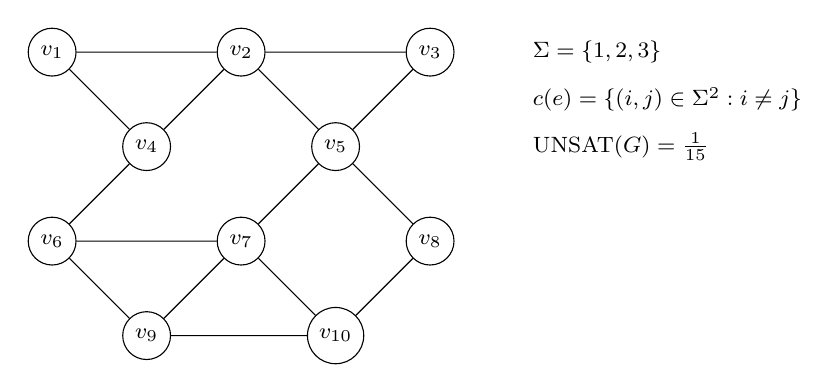
\begin{tikzpicture}[scale=1.2]
      % 頂点の定義
      \node[circle,draw,fill=white] (v1) at (0,3) {$v_1$};
      \node[circle,draw,fill=white] (v2) at (2,3) {$v_2$};
      \node[circle,draw,fill=white] (v3) at (4,3) {$v_3$};
      \node[circle,draw,fill=white] (v4) at (1,2) {$v_4$};
      \node[circle,draw,fill=white] (v5) at (3,2) {$v_5$};
      \node[circle,draw,fill=white] (v6) at (0,1) {$v_6$};
      \node[circle,draw,fill=white] (v7) at (2,1) {$v_7$};
      \node[circle,draw,fill=white] (v8) at (4,1) {$v_8$};
      \node[circle,draw,fill=white] (v9) at (1,0) {$v_9$};
      \node[circle,draw,fill=white] (v10) at (3,0) {$v_{10}$};
      
      % 辺の定義
      \draw (v1) -- (v2) -- (v3) -- (v5) -- (v2);
      \draw (v1) -- (v4) -- (v2);
      \draw (v4) -- (v6) -- (v7) -- (v5);
      \draw (v7) -- (v9) -- (v10) -- (v8) -- (v5);
      \draw (v6) -- (v9);
      \draw (v7) -- (v10);
      
      % 凡例
      \node[anchor=west] at (5,3) {$\Sigma = \{1,2,3\}$};
      \node[anchor=west] at (5,2.5) {$c(e) = \{(i,j) \in \Sigma^2 : i \neq j\}$};
      \node[anchor=west] at (5,2) {$\mathrm{UNSAT}(G) = \frac{1}{15}$};
    \end{tikzpicture}
    \caption{3彩色問題の制約グラフの例. 各頂点は3色のいずれかで彩色される必要があり, 隣接する頂点は異なる色でなければならない. この例では最適な彩色でも少なくとも1つの辺の制約を違反する必要があり, その割合は$\frac{1}{15}$となる.}
    \label{fig:3-coloring-constraint-graph}
  \end{figure}

\subsection{前処理補題}

PCP定理の証明の最初のステップは, 任意のCSPインスタンスを制約グラフに変換する前処理補題である. この変換は, 元のCSPの充足可能性と不満足値の基本的な性質を保持しつつ, 制約グラフの形式に変換する.

\begin{lemma}{前処理補題}{preprocessing-lemma}
  任意の$q$-CSPインスタンス$\varphi$に対して, 以下の性質を満たす制約グラフ$G$を多項式時間で構築できる:
  \begin{itemize}
  \item $\varphi$がYesインスタンスであることと, $\mathrm{UNSAT}(G) = 0$であることは同値である.
  \item $\varphi$がNoインスタンスであるとき, $\mathrm{UNSAT}(G) \ge \frac{1-\val(\varphi)}{q}$である.
  \item グラフ$G$の頂点数は$\abs{V} = O(n)$である.
  \item グラフ$G$の辺数は$\abs{E} = O(m)$である.
  \item アルファベット$\Sigma$は元のCSPと同じである.
  \end{itemize}
\end{lemma}

この補題の証明は, CSPインスタンスの制約を辺の制約に変換する単純な構築法に基づく. 具体的には, 各制約$c_i$に対して, その制約に含まれる変数間の辺を追加し, その辺に制約$c_i$を付随させる. この変換により, CSPの充足可能性と不満足値の基本的な性質が保持される.

前処理補題は, 任意のCSPインスタンスを制約グラフの形式に変換することで, 以降のギャップ増幅ステップのための準備を行う. この変換は多項式時間で実行可能であり, 元のCSPの重要な性質を保持するため, PCP定理の証明の基礎となる.

\section{エクスパンダーグラフ}
\subsection{エクスパンダーグラフの定義}

エクスパンダーグラフは, グラフの接続性を定量的に表現する重要な概念である. 特に, 任意の部分集合に対して, その境界のサイズが部分集合のサイズに応じて十分大きいという性質を持つ.

\begin{definition}{エクスパンダーグラフ}{expander-graph}
  $d$-正則グラフ$G=(V,E)$が\emph{$(n,d,\lambda)$-エクスパンダー}であるとは, 以下の条件を満たすことである:
  \begin{itemize}
  \item $\abs{V}=n$である.
  \item 任意の頂点の次数が$d$である.
  \item 任意の$S\subseteq V$に対して, $\abs{S}\le n/2$のとき
    \begin{align*}
      \abs{E(S,\overline{S})} \ge \lambda \cdot d \cdot \abs{S}
    \end{align*}
    が成り立つ. ここで, $E(S,\overline{S})$は$S$と$\overline{S}$を結ぶ辺の集合である.
  \end{itemize}
\end{definition}

エクスパンダーグラフの重要な性質として, ランダムウォークの収束が速いことが知られている. これは, エクスパンダーグラフのスペクトルギャップが大きいことと密接に関連している.

\subsection{エクスパンダー混交補題}

エクスパンダー混交補題は, エクスパンダーグラフにおけるランダムウォークの収束性を定量的に表現する重要な結果である.

\begin{lemma}{エクスパンダー混交補題}{expander-mixing-lemma}
  $(n,d,\lambda)$-エクスパンダー$G=(V,E)$を考える. 任意の$S,T\subseteq V$に対して
  \begin{align*}
    \abs{E(S,T)} - \frac{d}{n}\abs{S}\abs{T} \le \lambda\sqrt{\abs{S}\abs{T}}
  \end{align*}
  が成り立つ.
\end{lemma}

\begin{proof}
  隣接行列$A$の固有値を$\lambda_1\ge\lambda_2\ge\cdots\ge\lambda_n$とする. このとき, $\lambda_1=d$であり, $\lambda_2\le\lambda$であることが知られている.
  
  任意の$S,T\subseteq V$に対して, 特性ベクトル$\chi_S,\chi_T$を考える. このとき
  \begin{align*}
    \abs{E(S,T)} = \chi_S^\top A\chi_T
  \end{align*}
  が成り立つ. また, $\chi_S$と$\chi_T$を$A$の固有ベクトルで展開すると
  \begin{align*}
    \chi_S = \sum_{i=1}^n \alpha_i v_i, \quad \chi_T = \sum_{i=1}^n \beta_i v_i
  \end{align*}
  となる. ここで, $v_i$は$A$の固有ベクトルである.
  
  このとき
  \begin{align*}
    \abs{E(S,T)} - \frac{d}{n}\abs{S}\abs{T} &= \chi_S^\top A\chi_T - \frac{d}{n}\abs{S}\abs{T} \\
    &= \sum_{i=1}^n \lambda_i\alpha_i\beta_i - \frac{d}{n}\abs{S}\abs{T} \\
    &= \sum_{i=2}^n \lambda_i\alpha_i\beta_i \\
    &\le \lambda\sum_{i=2}^n \abs{\alpha_i\beta_i} \\
    &\le \lambda\sqrt{\sum_{i=2}^n \alpha_i^2}\sqrt{\sum_{i=2}^n \beta_i^2} \\
    &\le \lambda\sqrt{\abs{S}\abs{T}}
  \end{align*}
  が成り立つ.
\end{proof}

エクスパンダー混交補題は, エクスパンダーグラフにおける辺の分布が一様であることを示している. これは, PCP定理の証明において, 制約システムの不満足値を増幅する際に重要な役割を果たす.

\section{制約グラフのエクスパンダー化}

制約グラフのエクスパンダー化は, PCP定理の証明における重要なステップである. この変換により, 制約グラフの不満足値を増幅することが可能となる.

\begin{lemma}{制約グラフのエクスパンダー化}{constraint-graph-expander}
  制約グラフ$G=\langle(V,E),\Sigma,C\rangle$に対して, 以下の性質を満たす制約グラフ$G'=\langle(V',E'),\Sigma,C'\rangle$を多項式時間で構築できる:
  \begin{itemize}
  \item 基礎グラフ$(V',E')$は$(n',d',\lambda')$-エクスパンダーである. ここで, $n'=O(n)$, $d'=O(1)$, $\lambda'=O(1/\sqrt{d'})$である.
  \item $\mathrm{UNSAT}(G') \ge \Omega(\mathrm{UNSAT}(G))$である.
  \item アルファベット$\Sigma$は元のグラフと同じである.
  \end{itemize}
\end{lemma}

\begin{proof}
  制約グラフ$G$をエクスパンダーに変換する方法を説明する. 主なアイデアは, グラフの冪乗操作を用いて接続性を向上させることである.

  \emph{グラフの冪乗操作:}
  制約グラフ$G$の$t$乗$G^t$を以下のように定義する:
  \begin{itemize}
  \item 頂点集合は元のグラフと同じ$V$である.
  \item 辺$(u,v)$は, $G$上で$u$から$v$への長さ$t$のパスが存在する場合に存在する.
  \item 各辺$e'$の制約$c'(e')$は, 対応するパス上の制約の合成である. すなわち, パス$e_1,\dots,e_t$に対して
    \begin{align*}
      c'(e') = \{(a,b) \in \Sigma^2 : \exists a_1,\dots,a_{t-1} \in \Sigma, (a,a_1) \in c(e_1), (a_1,a_2) \in c(e_2), \dots, (a_{t-1},b) \in c(e_t)\}
    \end{align*}
    と定義する.
  \end{itemize}

  この冪乗操作により, グラフの接続性が向上し, エクスパンダー性が得られる. 具体的には, 以下の性質が成り立つ:

  \begin{lemma}{}{}
    制約グラフ$G$の$t$乗$G^t$は, 元のグラフ$G$の接続性を$t$倍に増幅する. すなわち, 任意の$S\subseteq V$に対して
    \begin{align*}
      \abs{E_{G^t}(S,\overline{S})} \ge t \cdot \abs{E_G(S,\overline{S})}
    \end{align*}
    が成り立つ.
  \end{lemma}

  \begin{proof}[Lemmaの証明]
    任意の$S\subseteq V$を考える. $G$上の$S$と$\overline{S}$を結ぶ辺の数を$k$とする.
    このとき, $G^t$上では, これらの辺を通る長さ$t$のパスが少なくとも$k$個存在する.
    各パスは$G^t$上の辺に対応するため, $E_{G^t}(S,\overline{S})$のサイズは少なくとも$k$である.
  \end{proof}

  次に, 不満足値の関係を証明する:

  \begin{lemma}{}{}
    $\mathrm{UNSAT}(G^t) \ge \Omega(t \cdot \mathrm{UNSAT}(G))$が成り立つ.
  \end{lemma}

  \begin{proof}[Lemmaの証明]
    任意の割り当て$\sigma: V \rightarrow \Sigma$を考える. $G$上の不満足な辺の割合を$\epsilon$とする.
    このとき, $G^t$上の任意の辺$e'$は, $t$個の$G$上の辺の制約の合成である.
    これらの制約のうち少なくとも$\epsilon t$個が不満足であるため,
    $\mathrm{UNSAT}_{\sigma}(G^t) \ge \Omega(\epsilon t)$が成り立つ.
  \end{proof}

  最後に, 適切な$t$を選択することで, 所望のエクスパンダー性が得られることを示す.
  $t=O(\log n)$とすると, グラフ$G^t$は$(n',d',\lambda')$-エクスパンダーとなる.
  ここで, $n'=n$, $d'=d^t=O(1)$, $\lambda'=O(1/\sqrt{d'})$である.
\end{proof}

この補題により, 任意の制約グラフをエクスパンダーに変換しつつ, 不満足値を保持することができる.
これは, PCP定理の証明におけるギャップ増幅ステップの基礎となる.
\chapter{ギャップ増幅補題} \label{chap:gap-amplification}

DinurによるPCP定理の証明は, 与えられた制約グラフの不満足値を段階的に増幅していくアプローチに基づく.
その中核を担うのがこのギャップ増幅補題であり, 制約グラフの不満足値を増幅できることを保証する補題である.
本チャプターはこの補題の証明を与える.

\section{主張}
ギャップ増幅補題は以下のように述べられる.

\begin{lemma}{ギャップ増幅補題}{gap-amplification-lemma}
  二つの定数$C>0,\alpha\in (0,1)$および, 
  制約グラフ$G=\ip{(V,E),\Sigma,\calC}$を入力として受け取り, 以下の性質を満たす別の制約グラフ$G'=\ip{(V',E'),\Sigma,\calC'}$を出力する決定的多項式時間アルゴリズムが存在する:
  \begin{itemize}
    \item $\size(G')\le C\cdot \size(G)$.
    \item $\UNSAT(G)=0$ならば$\UNSAT(G')=0$.
    \item $\UNSAT(G)>0$ならば$\UNSAT(G')\ge \min\{\alpha, 2\cdot \UNSAT(G)\}$.
  \end{itemize}
\end{lemma}

PCP定理(\cref{thm:PCP-CSP-theorem})の証明は, この補題を繰り返し適用することによって得られる.

\begin{proof}[\cref{lem:gap-amplification-lemma}の下での\cref{thm:PCP-CSP-theorem}の証明.]
  3彩色問題のインスタンスを入力として受け取り, その制約グラフを$G_0$とし, 頂点数を$n$とする.
  この制約グラフは単純グラフであるため, $\UNSAT(G_0)=0$もしくは$\UNSAT(G_0)\ge \frac{1}{n^2}$である.
  \cref{lem:gap-amplification-lemma}のアルゴリズムを$A$とし, 各$i=1,\dots,\ceil{2\log_2 n}$について, 制約グラフ$G_i$を
  $G_i = A(G_{i-1})$として定義し, 最終的に得られる制約グラフを$G'=G_{\ceil{2\log_2 n}}$とする.
  各$G_i$のサイズは$\size(G_i) \le C\cdot \size(G_{i-1})$であるため, $\size(G')\le C^{\ceil{2\log_2 n}}\cdot \size(G_0)=\size(G_0)^{O(1)}$である.
  従って$G'$は多項式時間で構成できる.

  また, 不満足値については, 以下のようになる:
  \begin{itemize}
  \item もしも$G_0$がYesインスタンスであるならば, 全ての$i$に対して$G_i$もYesインスタンスであり, 特に$\UNSAT(G')=0$である.
  \item もしも$G_0$がNoインスタンスであるならば, $\UNSAT(G_0)\ge \frac{1}{n^2}$かつ$\UNSAT(G_i)\ge \min\{\alpha, 2\cdot \UNSAT(G_0)\}$であるため, $\UNSAT(G')\ge \min\qty{\alpha, 2^{2\log_2 n}\cdot \frac{1}{n^2}}=\alpha$である.
  \end{itemize}
\end{proof}

\section{証明の概要}

\section{エクスパンダー化}

\subsection{エクスパンダーグラフとその性質}

\subsection{制約グラフのエクスパンダー化}

\section{冪乗操作}

\section{アルファベット削減}




\chapter{アルファベット削減} \label{chap:alphabet-reduction}

\section{PCP定理の証明}

PCP定理の証明の最後のステップは, アルファベットサイズを定数に削減することである. これは, ギャップ増幅ステップによって増加したアルファベットサイズを, 標準的なPCP合成ステップを用いて修正する.

\begin{lemma}{アルファベット削減補題}{alphabet-reduction-lemma}
  定数$\epsilon > 0$が存在し, 以下の性質を満たす多項式時間アルゴリズムが存在する:
  入力として制約グラフ$G = \langle(V, E), \Sigma, C\rangle$を受け取り, 新しい制約グラフ$G' = \langle(V', E'), \Sigma', C'\rangle$を出力する.
  \begin{itemize}
  \item $\mathrm{UNSAT}(G) = 0$ならば$\mathrm{UNSAT}(G') = 0$である.
  \item $\mathrm{UNSAT}(G) > 0$ならば$\mathrm{UNSAT}(G') \ge \min(\mathrm{UNSAT}(G), \epsilon)$である.
  \item $\abs{V'} = O(\abs{V})$である.
  \item $\abs{E'} = O(\abs{E})$である.
  \item $\abs{\Sigma'} = O(1)$である.
  \end{itemize}
\end{lemma}

この補題の証明は, 標準的なPCP合成ステップを用いる. 具体的には:

\begin{enumerate}
\item \textbf{制約の分解}: 各制約$c(e)$を, より小さなアルファベットサイズを持つ制約の集合に分解する.

\item \textbf{制約の合成}: 分解された制約を, 新しい制約グラフ$G'$の制約として合成する.

\item \textbf{正当性の証明}: 元の制約グラフと新しい制約グラフの不満足値の関係を証明する.
\end{enumerate}

このアルファベット削減補題は, PCP定理の証明の最後のピースとなる. これにより, 制約グラフのアルファベットサイズを定数に削減しつつ, 不満足値の基本的な性質を保持することができる.

\section{まとめ}

PCP定理の証明は, 以下の3つの主要なステップから構成される:

\begin{enumerate}
\item \textbf{前処理補題}: 任意のCSPインスタンスを制約グラフに変換する.

\item \textbf{ギャップ増幅補題}: 制約グラフの不満足値を2倍に増幅する.

\item \textbf{アルファベット削減補題}: アルファベットサイズを定数に削減する.
\end{enumerate}

これらの補題を組み合わせることで, PCP定理が証明される. この証明は, 制約システムの不満足値という量に着目することで, より直接的にPCP定理を証明できる点に特徴がある.
%\chapter{誤り訂正符号} \label{chap:error-correcting code}
誤り訂正符号とは文字列に冗長性を付加してノイズに対する頑健性を達成する手法である.
厳密には, \emph{アルファベット}と呼ばれる有限集合$\Sigma$上の文字列$x \in \Sigma^n$を受け取り, より長い文字列
%\input{expander graph.tex}
%\input{HDX.tex}
%\input{matroid.tex}
\printbibliography
\appendix
\chapter{付録}

\section{基本的な確率の不等式}
この節では, 証明の中で用いられる確率の不等式とその証明を述べる.
\begin{lemma}{Markovの不等式}{markov-inequality}
  任意の非負の確率変数$X$と任意の$t>0$に対し,
  \begin{align*}
    \Pr[X\ge t] \le \frac{\E[X]}{t}
  \end{align*}
  が成り立つ.
\end{lemma}

\begin{proof}
  ここでは簡単のため, $X$の台$\Omega=\supp(X)\subseteq\Real$は有限集合, すなわち$\abs{\Omega}<\infty$と仮定する\footnote{確率変数$X$のとりうる値の集合, すなわち$\qty{x\colon \Pr[X=x]>0}$を$X$の台と呼び, $\supp(X)$と表す.}.
  このとき,
  \begin{align*}
    \E[X] = \sum_{x\in \Omega} x\Pr[X=x] \ge \sum_{x\in \Omega,x\ge t} x\Pr[X=x] \ge \sum_{x\in \Omega,x\ge t} t\Pr[X=x] = t\Pr[X\ge t]
  \end{align*}
  を整理すると主張を得る.
\end{proof}

\begin{lemma}{Chebyshevの不等式}{chebyshev-inequality}
  期待値$\E[X]$と分散$\Var[X]$が存在する任意の確率変数$X$と任意の$t>0$に対し,
  \begin{align*}
    \Pr[|X-\E[X]|\ge t] \le \frac{\Var[X]}{t^2}
  \end{align*}
  が成り立つ.
\end{lemma}
\begin{proof}
  確率変数$Y=(X-\E[X])^2$は非負の確率変数であるから, これにMarkovの不等式を適用すると
  \begin{align*}
    \Pr\qty[ \abs{X - \E[X]} \ge t  ] &= \Pr\qty[ (X-\E[X])^2 \ge t^2 ] \\
    &\le \frac{\E\qty[ (X-\E[X])^2 ]}{t^2} \\
    & = \frac{\Var[X]}{t^2}
  \end{align*}
  を得る.
\end{proof}

\begin{lemma}{Paley-Zygmundの不等式}{paley-zigmund-inequality}
  非負整数値をとる任意の確率変数$X$に対し,
  \begin{align*}
    \Pr[X\ge 1] \ge \frac{\E[X]^2}{\E[X^2]}.
  \end{align*}
\end{lemma}
\begin{proof}
  非負整数値をとる確率変数$X$に対し
  \begin{align*}
    \E[X] &= \E[X\cdot \indicator{X\ge 1}] \\
    &\le \sqrt{ \E[X^2]\cdot \E[\indicator{X\ge 1}] } & & \because\text{Cauchy-Schwarzの不等式}\\
    &= \sqrt{ \E[X^2]\cdot \Pr[X\ge 1] }.
  \end{align*}
  両辺を二乗して整理すると主張を得る.  
\end{proof}
\end{document}